\section{Experimental Evaluation}
\label{sec:evaluation}

Here we present all of our experiments.

\begin{table*}[t]
\centering
\caption{Accuracy of different speech recognition services and accents against every audio captcha service we evaluated.}
\begin{tabular}{lccccc}
\toprule
&\multicolumn{5}{c}{\textbf{Speech Recognition Service (Accent)}}\\
\cmidrule{2-6}
\textbf{Captcha Service}& \textbf{Wit}& \textbf{IBM (US)} & \textbf{ IBM (UK)} & \textbf{Google (US)} & \textbf{Google (UK)} \\
\hline
Recaptcha v2.a &  &  & & & \\
\rowcolor{Gray}
Recaptcha v2.b &  &  &  & & \\
Apple  &  & 2.3\% (6/260) & 6.8\% (17/251) & 35.8\% (126/352) & \textbf{52.8\%} (143/271) \\
\rowcolor{Gray}
BotDetect  &  & &  & & \\
Captchas.net  & &  &  & & \\
\rowcolor{Gray}
Microsoft Live & &  &  & & \\
SecurImage  &  & &  & & \\
\rowcolor{Gray}
Telerik  & 21\% (142/670)  & \textbf{97\%} (452/466) & 12.7\% (47/364) & 74.4\% (150/202) & 51.6\% (112/217) \\
\end{tabular}
\label{tab:combinations}
\end{table*}


\note{Rate limit of speech recognition services.}

\begin{figure*}
\centering
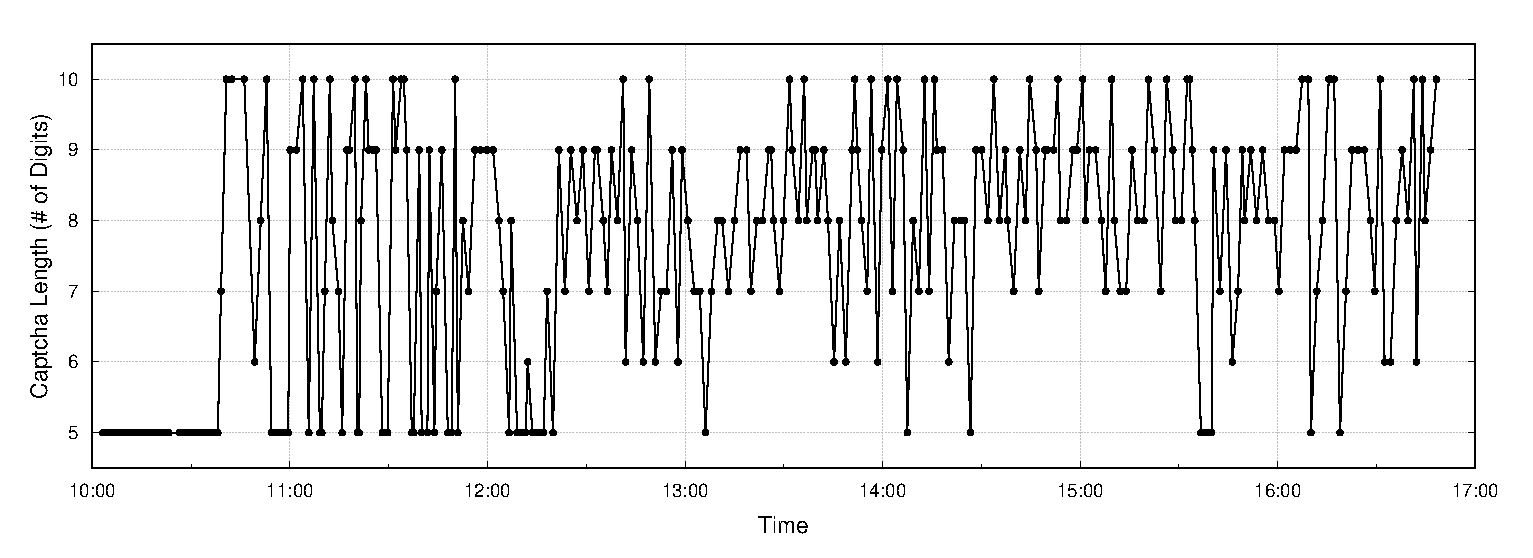
\includegraphics[width=0.8\textwidth]{figures/captcha_length.eps}
\caption{Variation of audio captcha length in \re v2.a over time.}
\label{fig:length}
\end{figure*}

\note{Length of audio captcha}
While by default the length of \re is 5 digits, we found that after multiple captcha solutions by our system,
\re would randomly return captchas with more digits. In Figure~\ref{fig:length} we present a representative experiment.

\note{Time to solve captcha per speech service}

\note{How many mistakes allowed for a correct answer?}

\note{economic analysis: length of challenge, cost per minute for solver. reselling solved tokens. How much profit?}

\note{plot length of recaptcha over time, similar to number of captchas per cookie from eurosp paper.}

